%Documento elaborado através da modificação de Template_ Tese_ MAEG por RJF. 
%Com contribuições e modificações dos alunos do DEGGE e Phd student 
%Angelo Soares (arsoares@fc.ul.pt) com orientação de Carla M. Silva.
%11/11/2021
% Para escrever neste documento, expandam a secção Capitulos e escrevam no capitulo apropriado.
% Após a escrita, seleccionem "main.tex" e recompilem. Tudo o que escreverem nos capitulos irá 
% aparecer. 

% ------------------------------------------------------------------------------------------------------%
% ------------------------------------------ ALTERAR CAPA ----------------------------------------------%
% ------------------------------------------------------------------------------------------------------%
%A Neste main.tex as únicas alterações que precisam de fazer são referentes à Capa da
%dissertação. Sigam as indicações seguintes: Façam ctrl+F para procurar "includepdf" e leiam 
%as notas por baixo do \includepdf.

% ------------------------------------------------------------------------------------------------------%

%Outras Notas: 
%1. Ler o conteudo em "library.bib".
%2. O GOOGLE é vosso amigo, todas e quaisquer modificações necessárias, seja para introduzir um
%certo tipo de formatação, seja para colocar uma figura ou tabela com especificações particulares,
%usem o GOOGLE, existem N exemplos para todo o tipo de alteração em latex. Com quase copy+paste
%code.
% ------------------------------------------ IMPORTANTE -----------------------------------------------%
%3. Neste documento existem algumas colisoes de pacotes, nomeadamente o tocloft e o book report
%e a maneira %como o chapter foi elaborado. Exemplo: Se os alunos quiserem colocar o prefixo "1."
%antes da introdução, ou seja "1. Introdução". No Indice ficaria "1 1. Introdução".
%ALTERNATIVA: Escrevam a dissertação na totalidade. No fim, façam download do PDF (cliquem segundo
%Icone após o Recompile). Com esse ficheiro PDF, abram-no no PDF reader (adobe acrobat pro) e 
%editem acrescentando o número do capitulo para ficar igual ao que está no Indice "1. Introdução".
%É a forma mais simples de resolver.

%Se alguem por curiosidade encontrar outra solução usando o tocloft package, como por exemplo, 
%ocultar o número do capitulo no TOC sem usar \chapter* ou interferir com o hyperref enviem essa
%info para o email supramencionado, muito obrigado.
%Boa sorte


\documentclass[11pt,a4paper,twoside,openright]{book}
% ------------------------------------------------------------------------------------------------------%
% ------------------------------------------- PREAMBLE -------------------------------------------------%
% ------------------------------------------------------------------------------------------------------%
\usepackage{mathptmx} % Fonte mais próxima de Times New Roman
% Alterar margens do documento
\usepackage[margin=2.5cm]{geometry}
\renewcommand{\baselinestretch}{1.15}
\usepackage{setspace}
\usepackage{fancyhdr}
\pagestyle{fancy}
\renewcommand{\chaptermark}[1]{\markboth{\MakeUppercase{\thechapter. #1 }}{}}
\renewcommand{\sectionmark}[1]{\markright{\thesection\ #1}}
\fancyhf{}
\fancyhead[RO]{\small{\rightmark}}
\fancyhead[LE]{\small{\leftmark}}
\setlength{\headheight}{12pt}
\addtolength{\topmargin}{-10.5pt}
\fancyfoot[C]{\thepage}
\renewcommand{\headrulewidth}{0pt}
\renewcommand{\footrulewidth}{0pt}
\addtolength{\headheight}{0.5pt}
\fancypagestyle{plain}{
  \fancyhead{}
  \renewcommand{\headrulewidth}{0pt}
}

\usepackage[backend=biber, natbib=true, style=numeric, sorting=none]{biblatex} %Numeric style
%\usepackage[backend=biber,style=authoryear,maxcitenames=1,autocite=inline,natbib=true]{biblatex}
%\addbibresource{library} %O ficheiro .bib que a bibliografia vai usar
%\bibliography{library}
%\addbibresource{library.bib} %O ficheiro .bib que a bibliografia vai usar
%\bibliography{library.bib}
\addbibresource{library.bib}

%\bibliographystyle XXX
%\usepackage[numbers]{natbib}

% Package que permite incluir imagens
\usepackage{graphicx}

% Comentar para não incluir a lista de figuras e tabelas no índice
\usepackage[nottoc]{tocbibind}

% Para citar referências
%\usepackage{natbib}
%\setcitestyle{numbers}
%\bibliographystyle{humannat}
%\setcitestyle{authoryear}

%Indentar primeiro parágrafo
\usepackage{indentfirst}

% Incluir até à subsecção no índice
\setcounter{tocdepth}{3}
\setcounter{secnumdepth}{3}

% Permite remover os espaços entre itens
\usepackage{enumitem}

% Caption para imagens
\usepackage[font=footnotesize]{caption}

% Referenciar anexos
\usepackage[toc,page]{appendix}

%Adicionar pdfs
\usepackage{pdfpages}

%Alterar nome de capitulo para a referencia
\usepackage{fmtcount}
\usepackage{url}

%Para expressões Matemáticas
\usepackage{amsmath}
\usepackage{bm}

%Bibliotecas
%\usepackage{biblatex}
%\usepackage[portuguese]{babel} %Can be switched to english
\usepackage{csvsimple}
\usepackage[utf8]{inputenc}
\usepackage{float}
\raggedbottom
\usepackage{subcaption}
\usepackage{eurosym}
\usepackage{booktabs}
\usepackage[T1]{fontenc}
\usepackage{csquotes}
\usepackage{tabularx}
\usepackage[nottoc]{tocbibind}
%\usepackage[scaled]{helvet}
%\renewcommand*\familydefault{\sfdefault}

%Comando que cria abreviaturas usado no Nomenclatura
\newcommand{\abbreviations}[1]{%
\vspace{12pt}\noindent{\selectfont\textbf{Abreviaturas}\par\vspace{6pt}\noindent {\fontsize{9}{9}\selectfont #1}\par}}
%Criar Siglas
\newcommand{\siglas}[1]{%
\vspace{12pt}\noindent{\selectfont\textbf{Siglas e acrónimos}\par\vspace{6pt}\noindent {\fontsize{9}{9}\selectfont #1}\par}}
%Cria simbologia
\newcommand{\simbolos}[1]{%
\vspace{12pt}\noindent{\selectfont\textbf{Simbologia}\par\vspace{6pt}\noindent {\fontsize{9}{9}\selectfont #1}\par}}

\makeatletter
\def\cleardoublepage{\clearpage\if@twoside \ifodd\c@page\else
    \hbox{}
    \thispagestyle{plain}
    \newpage
    \if@twocolumn\hbox{}\newpage\fi\fi\fi}
\makeatother \clearpage{\pagestyle{plain}\cleardoublepage}

\providecommand{\keywords}[1]{\textbf{Keywords:} #1}
\providecommand{\keywordsP}[1]{\textbf{Palavras chave:} #1}

%Remover Chapter N on the header
\usepackage{titlesec}
\usepackage{lipsum}
\titleformat{\chapter}[display]
   {\normalfont\huge\bfseries}{\chaptertitlename\ \thechapter}{20pt}{\Huge}   
\titlespacing*{\chapter}{0pt}{-20pt}{40pt}
\titleformat{\chapter}[display]{\normalfont\bfseries}{}{0pt}{\huge}

%\numberwithin{section}{chapter}
\usepackage{multirow}
\usepackage{chngcntr}  
\usepackage{tocloft}
\usepackage[hidelinks]{hyperref}
%\counterwithout{figure}{chapter}
%\counterwithout{table}{chapter}

\renewcommand{\cftfigpresnum}{\textbf{Figura\ }}
\renewcommand{\cfttabpresnum}{\textbf{Tabela\ }}

\newlength{\mylenf}
\settowidth{\mylenf}{\cftfigpresnum}
\setlength{\cftfignumwidth}{\dimexpr\mylenf+1.5em}
\setlength{\cfttabnumwidth}{\dimexpr\mylenf+1.5em}

\sloppy

\makeatletter
\newcommand\listoftablesandfigures{%
    \chapter*{List of Tables and Figures}%
    \phantomsection
\@starttoc{lof}%
\bigskip
\@starttoc{lot}}
\makeatother

\PassOptionsToPackage{hyphens}{url}\usepackage{hyperref}

% ------------------------------------------------------------------------------------------------------%
% ------------------------------------------- END - PREAMBLE -------------------------------------------%
% ------------------------------------------------------------------------------------------------------%

\begin{document}


% Capa
\newpage
\thispagestyle{empty}

%\setmainfont[Path = fonts/]{arial_narrow.ttf} 

\centering{\fontsize{12.2}{14.4}\selectfont UNIVERSIDADE DE LISBOA}\\
\centering{\fontsize{12.2}{14.4}\selectfont FACULDADE DE CIÊNCIAS}\\
\centering{\fontsize{12.2}{14.4}\selectfont DEPARTAMENTO DE ENGENHARIA GEOGRÁFICA,GEOFÍSICA E ENERGIA}

\vspace{1.3cm}

\begin{figure}[h]
 \centering
 
\includegraphics[width = 6.99cm,height = 3.3cm]{Imagens/logo_fcul.png}
\end{figure}

\vspace{3.45cm}

%\setmainfont[Path = fonts/]{arial_narrow_bold.ttf}

\centering{\fontsize{17}{20.4}\selectfont \textbf{Participação da geração renovável no mercado de reservas de um sistema eléctrico}}

%\setmainfont[Path = fonts/]{arial_narrow.ttf}

\vspace{4cm}

\centering{\fontsize{14}{16.8}\selectfont João Pedro Passagem dos Santos}

\vspace{1.3cm}

%\setmainfont[Path = fonts/]{arial_narrow_bold.ttf}

\centering{\fontsize{13}{15.6}\selectfont \textbf{Mestrado em Engenharia da Energia e Ambiente}}\\

%\setmainfont[Path = fonts/]{arial_narrow.ttf}

%\centering{\fontsize{13}{15.6}\selectfont Especialização em Bioinformática}

\vspace{0.5cm}


\vspace{0.5cm}

\centering{\fontsize{13}{15.6}\selectfont Dissertação orientada por:}\\
\centering{\fontsize{13}{15.6}\selectfont Doutor Hugo Algarvio}\\
\centering{\fontsize{13}{15.6}\selectfont Professora Doutora Ana Estanqueiro}\\

\vspace{2.9cm}

\centering{\fontsize{14}{16.8}\selectfont 2023}

\label{Capa}



\let\cleardoublepage\clearpage


\clearpage \thispagestyle{empty}\mbox{}\clearpage

\frontmatter
% RESUMO
\newpage
\thispagestyle{plain}
\chapter{Resumo}
\justifying

A crescente penetração de fontes de energia renováveis variáveis no tempo, vRES, no sistema eléctrico, como a solar ou eólica, está a transformar significativamente os mercados de eletricidade, devido à sua natureza intermitente e imprevisível. Isso torna as previsões de produção e consumo de energia mais desafiantes, especialmente porque os mercados fecham entre 1 e 37 horas antes da entrega real da energia, podendo originar discrepâncias entre as energias contratadas e necessárias. Manter o equilíbrio entre a oferta e a procura em tempo real é vital para a segurança e estabilidade da rede, função que recai principalmente sobre os operadores de redes de transporte (TSO).\par
Os TSO utilizam mercados de reserva de energia, onde adquirem de forma simétrica potência secundária ascendente e descendente, com base em previsões de procura para as horas subsequentes. No entanto, essa abordagem é ineficaz face às flutuações das renováveis, levando à necessidade de ajustes mais dinâmicos e precisos.\par
Este trabalho propõe um estudo de parâmetros fórmula do TSO português para a previsão de reserva necessária ($\rho$), onde, usando os dados históricos horários no período de 2008 a 2023, é calculado o $\rho$ que apresente menor erro na previsão, atingindo erros inferiores a 5\%.\par
O presente trabalho propõe também um modelo \textit{machine learning} para calcular dinamicamente as reservas de potência secundária, utilizando dados operacionais abertos do TSO espanhol. O modelo foi treinado com dados no período de 2014 a 2023, e validado com dados de referência de 2019 a 2022. A metodologia proposta demonstra uma melhoria significativa na utilização das reservas de potência secundária, com um aumento de aproximadamente 47\% na eficiência das reservas ascendentes e cerca de 42\% nas reservas descendentes. Este avanço contribui para uma gestão mais eficiente e equilibrada do sistema elétrico, especialmente em cenários com elevada penetração de vRES.\par




\vspace{0.5cm} %adiciona um espaço de 0.5cm entre o texto e as palavras chave.

\keywordsP{sistemas de reserva, mercados de energia, redes neuronais, previsões}
%reparem que # necessita de um \ para que o latex o interprete correctamente como um caracter especial. Isto também acontece com % por exemplo.
\label{resumo}

%Abstract
\newpage
\thispagestyle{plain}
\chapter{Abstract}
The growing penetration of renewable energy sources, in the energy produtction markets, together with the paradigm shift in size and centralization of producers, brings instabilities and variability not in the scoope of current market models. \\

In turn, due to their less constante nature, these renewble producers have greater difficulties in making a profit in current models. \\

Forecast technologies are increasingly migrating to \emph{machine learning} models, with more accurate results. \\

This work proposes the application of neural network technologies to forecast forecast secondary reserve allocation bands, using data from the Iberian market. \\

\vspace{0.5cm} %adiciona um espaço de 0.5cm entre o texto e as palavras chave.

\keywordsP{reserve systems,energy markets, neural networks, forecast}
%notice that # requires a \ so that latex correctly interprets it as a special character. This also happens with % for example.
\label{abstract}

% AGRADECIMENTOS
\newpage
\thispagestyle{plain}
\chapter{Agradecimentos}
\justifying

Começo por agradecer à minha família, que me acompanhou sempre neste longo e atribulado percurso académico.\par
Agradeço a todos os amigos que me inspiraram e me fizeram crescer pessoal, profissional e academicamente.\par
Um agradecimento especial à Ana, pelo companheirismo, apoio, jantares e trabalho constante de me manter em rumo. \par
Por último agradeço aos meus orientadores, a professora Doutora Ana Estanqueiro pela forte inspiração e confiança, e em especial ao Doutor Hugo Algarvio, pelo apoio, liderança, paciência e disponibilidade durante todo o tempo de realização deste trabalho.\par

\vspace{10mm} %ele aceita diversos tipos units, neste caso 10mm, 0.1cm.

\flushleft{João Pedro Passagem dos Santos}
\label{agradecimentos}

%Nomenclatura
\newpage
\thispagestyle{plain}
\chapter{Nomenclatura}
Lista de siglas, acrónimos, abreviaturas e simbologia apresentadas por ordem alfabética.

%Utilizar sempre \\ para forçar a mudança de linha.
%Utilizar o & para forçar a mudança de "coluna", como numa tabela
\abbreviations{\noindent 
\begin{tabular}{@{}ll}
(A/F) & Relação mássica ar/combustível\\
pme	& Pressão média efectiva\\
vol & Volume\\
\end{tabular}
}

\siglas{\noindent 
\begin{tabular}{@{}ll}
ODS & Objetivos de Desenvolvimento Sustentável\\
vRES & variable Renewable Energy Systems\\
MIBEL & Mercado Ibérico de Eletricidade\\
APA	& Agência Portuguesa do Ambiente\\
EDP & Eletricidade De Portugal\\
NREL & National Renewable Energy Laboratory\\
\end{tabular}
}

\simbolos{\noindent 
\begin{tabular}{@{}ll}
A & Área\\
\(\eta\) & Eficiência\\
p & Pressão\\
T & Temperatura\\
\end{tabular}
}
%The use of \( \) avoids obscure compiling errors in latex when using certain mathematical notation symbols in a non-mathematical environment (text).
%https://tex.stackexchange.com/questions/510/are-and-preferable-to-dollar-signs-for-math-mode

%Nota: List of greek letters and others https://pt.overleaf.com/learn/latex/List_of_Greek_letters_and_math_symbols
\label{ch:nomenclatura}

% ÍNDICE
% ÍNDICE (Não é preciso fazer nada, faz update automaticamente)
\clearpage
\thispagestyle{plain}
\renewcommand{\contentsname}{Índice}
\tableofcontents
\clearpage
\thispagestyle{plain}
\listoffigures
\clearpage
\thispagestyle{plain}
\listoftables
\clearpage \thispagestyle{plain}\mbox{}\clearpage

\mainmatter
\setlength{\parindent}{15pt} %Comentar retira a indentação inicial nos chapters
\pagenumbering{arabic} %numeros em numeração árabe

% INTRODUÇÃO
\newpage
\thispagestyle{plain}
\chapter{Introdução}

\section{Enquadramento\label{se:enquadramento}}
Esta dissertação enquadra-se no âmbito do projeto \href{https://traderes.eu/}{TradeRES}, que visa o estudo de um sistema de mercado eléctrico capaz de atender às necessidades da sociedade num sistema quase totalmente renovável, tendo as características para se integrar nos \href{https://ods.pt/ods/}{ \gls{ODS}} \ref{fig:ODS}.\par
O estudo da acessibilidade das energias renováveis ao mercado vigente integra-se nos \gls{ODS} n$^{\circ}$7, “Energia Renováveis e Acessíveis”, indo directamente de encontro a um dos pontos deste objectivo: 7.2.1 “Peso das energias renováveis no consumo total final de energia”. Por meio deste objectivo, a participação das renováveis no mercado faz também cumprir, embora indiretamente, o objectivo n$^{\circ}$8 “Trabalho Digno e Crescimento Económico”, através do ponto 8.4, onde, neste último, é dada primazia à eficiência dos recursos globais no consumo e na produção. Esta contribuição indireta ocorre através da diminuição do uso de energias não limpas, justificadas por um maior uso das renováveis, melhorando a gestão de recursos, e baixando o consumo de recursos naturais não renováveis.\par
Por último, no âmbito do presente estudo, podemos igualmente incluir o objectivo n$^{\circ}$13, “Acção Climática”, no qual, referimos, não só a diminuição de consumo de recursos finitos, mas ainda, a melhor gestão de recursos renováveis, promovendo o planeamento e estratégias de combate a emissões de gases de efeito estufa.\par

\begin{figure}[h]
    \centering
    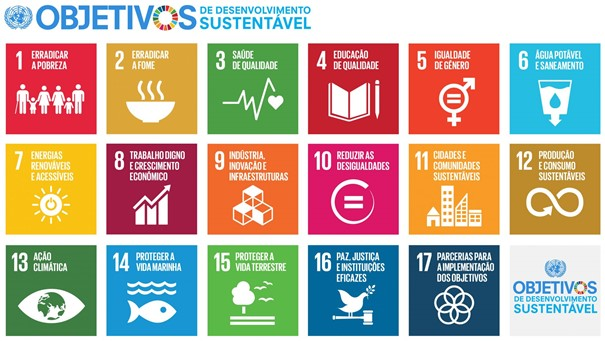
\includegraphics{Imagens/DesenvolvimentoSustentavel.jpg}
    \caption{Objectivos de Desenvolvimento Sustentável da ONU}
    \label{fig:ODS}
\end{figure}

\section{Objetivos e Perguntas de Pesquisa\label{se:objetivos}}

Foram aprovadas a nível europeu (2020)\cite{52020DC0299} sugestões de alterações aos serviços de sistema, que serão seguidas pelos Estados-Membros. Nesta dissertação, será realizada a aplicação dessas sugestões, identificando as melhorias em relação ao \textit{design} actual e avaliando se as novas sugestões serão suficientes para garantir a operação de um sistema elétrico \textasciitilde100\% renovável, potencialmente identificando ações adicionais para garantir a robustez e segurança do sistema elétrico sem o uso de combustíveis fósseis.\par
A penetração das \gls{vRES} no sistema de energia eléctrica trouxe maior incerteza na previsão em mercados de energia, pois estas estão mais sujeitos a elementos não controláveis como a velocidade do vento ou a radiação solar incidente.\par
As seguintes perguntas servirão de guia nesta pesquisa:\par

\begin{enumerate}[label=\alph*)]
  \item Podemos reduzir a incerteza na produção criada pela participação das \gls{vRES} nos sistemas de energia? 
  \item A alocação dinâmica pode ter um efeito positivo no mercado de reservas?
  \item É possível prever a necessidade de reserva necessária baixando a alocação desperdiçada?
\end{enumerate}

Para responder às perguntas \textit{supra} referidas, utilizaremos dados de previsão de geração de energia renovável para estimar a energia necessária para alocação secundária. Actualmente, os valores de previsão desse mercado estão distantes do consumo real, o que resulta em alocações no dia anterior que não estão em conformidade com as necessidades reais.\par
O objetivo deste trabalho é criar métodos de previsão para o dia seguinte, da necessidade de alocação de banda de reserva secundária, de modo a alocar banda suficiente e, simultaneamente, baixar a alocação em excesso, usando dados históricos das mesmas.\par
Iremos explorar a optimização da fórmula de alocação de banda de reserva da REN, testando novos valores para o parâmetro horário da mesma.\par
Utilizando técnicas de \textit{machine learning} vamos criar um modelo para a previsão de alocação necessária do dia seguinte.\par
Previsões mais exactas tornam possível uma melhor gestão das alocações, resultando num menor gasto de recursos energéticos e financeiros.\par

\section{Organização do Documento \label{se:organização}}

Este documento está dividido em capítulos. Sendo que os primeiros apresentam uma introdução às ideias e temas no 1, o estado de arte dos temas na literatura publicada, seguido de uma contextualização do tema do trabalho proposto no capítulo 2. Dentro da contextualização é de forma geral apresentado os mercados de energia, os sistemas de reserva, e os métodos de previsão para os mesmos, dentro destes o uso de fórmulas e o uso de \textit{machine learning}, formulando aqui a motivação e caminho de estudo.\par
No capítulo 3 apresentamos no sub-capítulo Ferramentas as bibliotecas criadas em \textit{python} para o presente estudo.
Segue o sub-capítulo Métodos onde abordamos os diferentes estudos presentes, como serão dirigidos e condições a alcançar. Dividindo o trabalho em estudos distintos para o tipo de previsões apresentadas no capítulo 2.
Métricas e Dados intitula o capítulo 4 que começa numa dissecção das métricas aplicadas ao longo das experiências e como estas influenciam a mesma, terminando num estudo geral dos dados utilizados, seus tratamentos e elações iniciais de análise. Apresentado também o que é usado como treino e como validação para as experiências.
No capítulo 5 são apresentados os resultados da experiência completa, incluindo as métricas apresentadas, apresentado gráficos de séries temporais das previsões conseguidas. Dando realce aos melhores modelos e optimizações conseguidos.
Termina com um breve capítulo conclusivo dando um pouco mais de contexto aos resultados, apresentando possíveis caminhos futuros de melhoria dos mesmos e discutindo o impacto de \textit{machine learning} no futuro das energias renováveis e consequentemente nos mercados de reserva.

% Os dois capítulos seguintes apresentam os dois diferentes estudos. No \hyperref[ch:estudo_1]{capítulo 4} é definido e apresentado o resultado do estudo da estimativa do parâmetro $\rho$ da fórmula de estimativa da \gls{REN}.\par
% No \hyperref[ch:estudo_2]{capítulo 5} explora-se o segundo estudo, o dimensionamento dinâmico da alocação necessária. São apresentados os dados utilizados com um estudo preliminar sobre os mesmos, e o tratamento necessário para usar nos modelos.\par
% No \hyperref[ch:ferramentas]{capítulo 6} as ferramentas de programação criadas para realizar a mesma.\par
% Os 3 capítulos seguintes são os descritivos da experiência em si. \hyperref[ch:metricas]{Capítulo 7} são as métricas usadas e criadas para a validação da experiência, \hyperref[ch:metodos]{capítulo 8} é a estrutura e parametrização da mesma, e \hyperref[ch:resultados_discussao]{capítulo 9} apresenta os resultados.\par
% Termina com um \hyperref[ch:conclusao]{capítulo conclusivo} onde são avaliadas as experiências como um todo, e o seu impacto no âmbito dos mercados de reserva.\par
\label{ch:intro}

% Revisão bibliográfica
\newpage
\thispagestyle{plain}
\chapter{Revisão bibliográfica}

A revisão bibliográfica deve recorrer a normas, livros, artigos científicos e, obrigatoriamente, deve indicar a bibliografia consultada de forma correta com recorrência a um reference manager. A maneira mais usual é adotar o sistema numerado por ordem de aparecimento do texto.\\
Isto é um exemplo de uma equação:

\begin{equation}
\label{eq:eq1}
    a = 1
\end{equation}

A tabela deve ter uma legenda por cima da mesma, tal como o exemplo em baixo. Se os valores da tabela não são calculados pelo autor e referem-se a valores de outros autores tem de constar as respetivas referências aos seus trabalhos.

%Tabela construida com https://www.tablesgenerator.com/

%Para ter a citação em formato [1] usem \cite{}
%Para usar citet ou citep teriam de modificar o style do \usepackage[backend=biber, natbib=true, style=numeric, sorting=none ]{biblatex} style de numerico para authoryear


\label{ch:revisao}

% Contextos
\newpage
\thispagestyle{plain}
\chapter{Contextos\label{ch:contextos}}

\section{Mercado de Serviços de Sistema \label{se:servicos_sistema}}
%\cite{Lopes2021}
%\cite{Watson1984}
%\citep{Schweppe1988}

O mercado de serviço de sistema é parte integrante dos mercados de energia e mantêm responsabilidade sobre a segurança do mesmo.\cite{dgegmss} \\
Serve para garantir o equilibrio entre a energia produzido e a consumida. Esta qualidade e segurança é controlada através da frequência e da potência activa, controlo de tensão e potência reactiva, arranque automático e outras técnicas de sistemas \cite{Rassid2017} \cite{Carneiro2016}. \\
Neste caso de estudo estamos interessados nos serviçoes de controlo de frequência. A nível europeu estes serviços são impostos pela ENTO-E (\textit{European Network of Transmission System Operators for Electricity}), e a operação dos mesmos é da responsabilidade dos TSO (\textit{Transmission System Operator} ou \textit{ Operador da Rede de Transporte}) nacionais.\\
Para manter o controlo de frequência o gestor de sistema deverá manter reservas para responder às diferenças entre a energia consumida e produzida na rede, que deve ser mantida em equilibrio. Quando o serviço de sistema precisa de actuar para manter a frequência no seu valor nominal, 50Hz na Europa, isto é feito alterando a potência activa dos geradores.  \\
Quando é necessário um aumento na potência chama-se a isto Banda de Reserva/Regulação a Subir, e quando é necessária uma diminuição chama-se à mesma a Descer. \\
Para isto, mo mercado ibérico, a tarefa é dividida em três reservas, primária, secundária e terciária. Esta divisão assenta no tempo de resposta que os sistemas precisam de ter, e na capacidade de actuação (MWh/Hz). \\

A reserva secundária, como sistema de segurança à reserva primária, regula-se pelo mercado de banda das reservas secundárias, que decorre no dia anterior ao que será necessário utilização da mesma. \\
Este valor alocado tem um custo para as operadoras, como tal a previsão do mesmo é importante para a gestão destes sistemas de segurança. Estas previsões são feitas através de estatiscas dos sistemas, e tendo em conta as areas de balanço que o mesmo têm. \\
Uma melhor previsão deste valor poderia levar a uma poupança, tanto financeira, como de recursos. \\

Estas previsões são feitas ao uso de formulas. Que por si só não preveêm a variabilidade dos sistemas de produção de energia renovável. Esta variabilidade sendo dificilmente previsivel, tem sido alvo de estudo com modelos de \textit{machine learning} \cite{} \\
Com bons resultados apresentados em estudo de energias renováveis, a aplicação dos mesmos metódos para as reservas de sistema parece um passo natural. \\



%\section{MIBEL \label{se:mibel}}
%\cite{Bessa2012}
%\cite{Carneiro2016}
%\cite{Fernandes2016}
%\citep{Agostini2021}


\label{ch:contexto}

% Dados
\newpage
\thispagestyle{plain}
\chapter{Dados}

\section{Dados Utilizados \label{se:dados_crus}}

Os dados em estudo são do mercado energético espanol, retirados do site :
https://www.esios.ree.es/es


\csvautotabular{../data/indicators_metadata.csv}


\subsection{Aquisição dos Dados (depth 2)}

No ambito da automatização destes dados foi modificado o repositorio ESIOS (creditar, como?) para ser usado como uma biblioteca de python, aberta, em pypi.
Sendo uma ferramenta mais facilmente acessivel para a extrair dados do mercado espanhol:
https://pypi.org/project/pyesios/



\section{Estudo dos dados  \label{se:dados_estudo}}

Os dados que propunho a prever são: "UpwardUsedSecondaryReserveEnergy", "DownwardUsedSecondaryReserveEnergy"

\begin{figure}[H]
  \centering
  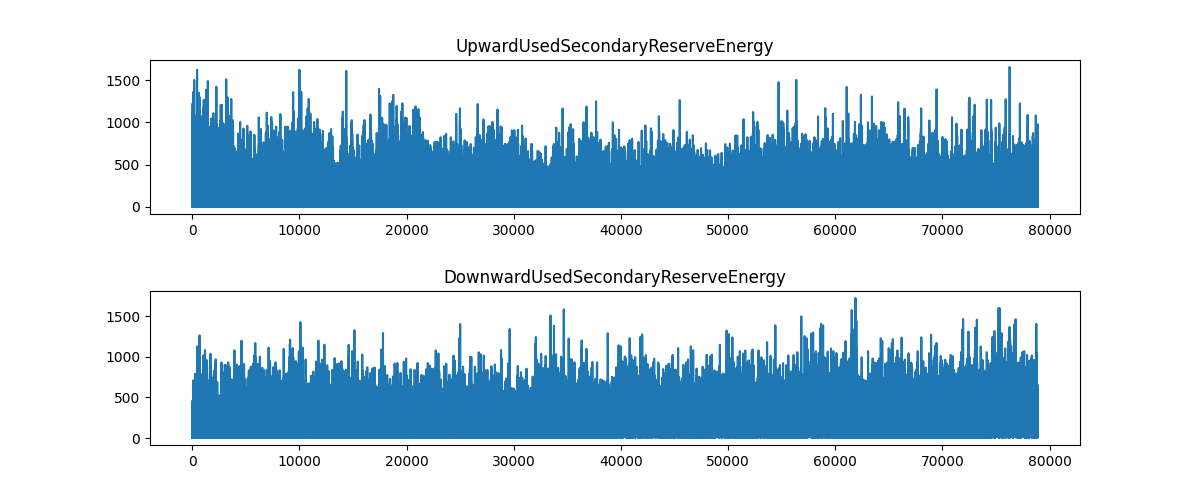
\includegraphics[width=0.8\textwidth]{../plots/targets_timeseries.png}
  \caption{Serie Temporal dos dados alvo}
  \label{fig:target_timeseries}
\end{figure}

Para termos uma melhor percepção dos mesmos segue algumas janelas temporais mais pequenas.

\begin{figure}[H]
  \centering
  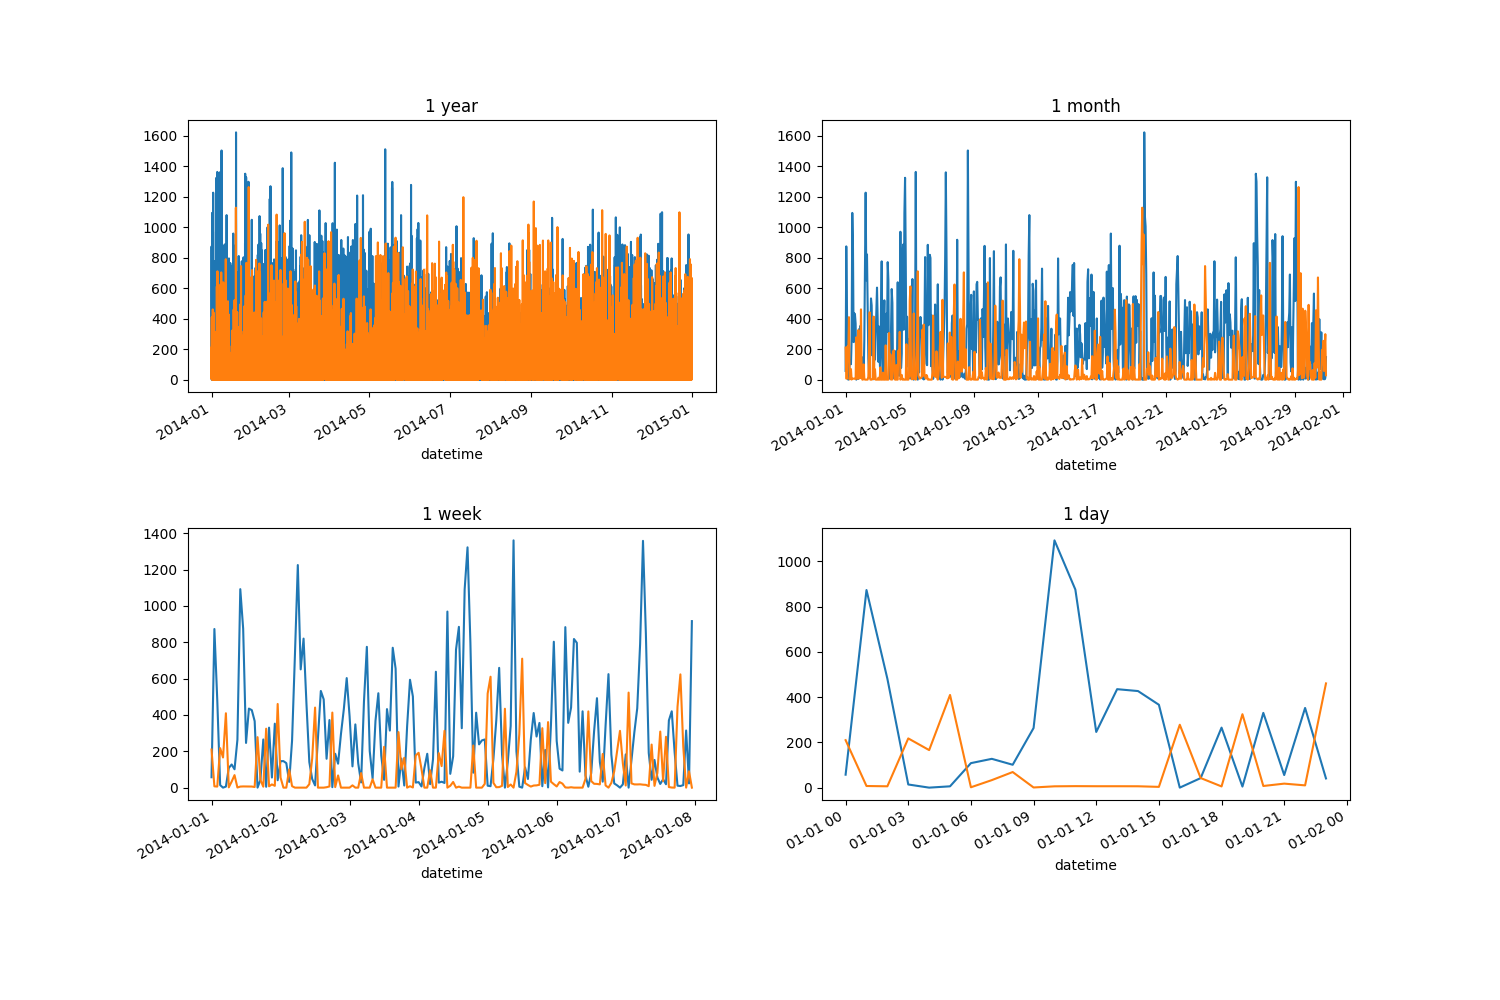
\includegraphics[width=0.8\textwidth]{../plots/target_timeseries_windows.png}
  \caption{Janelas Temporais dos dados alvo}
  \label{fig:target_timeseries_windows}
\end{figure}


Estas mostram claramente que ambos os atributos mantêm um comportamento tanto discreto, como linear, isto é, que ou existe algum valor, ou é zero, e se existe valor este tem comportamento linear.



A distribuição destes dados é claremente exponencial. O que é importante para a escolha de alguns parametros no modelação

		
\begin{figure}[H]
  \centering
  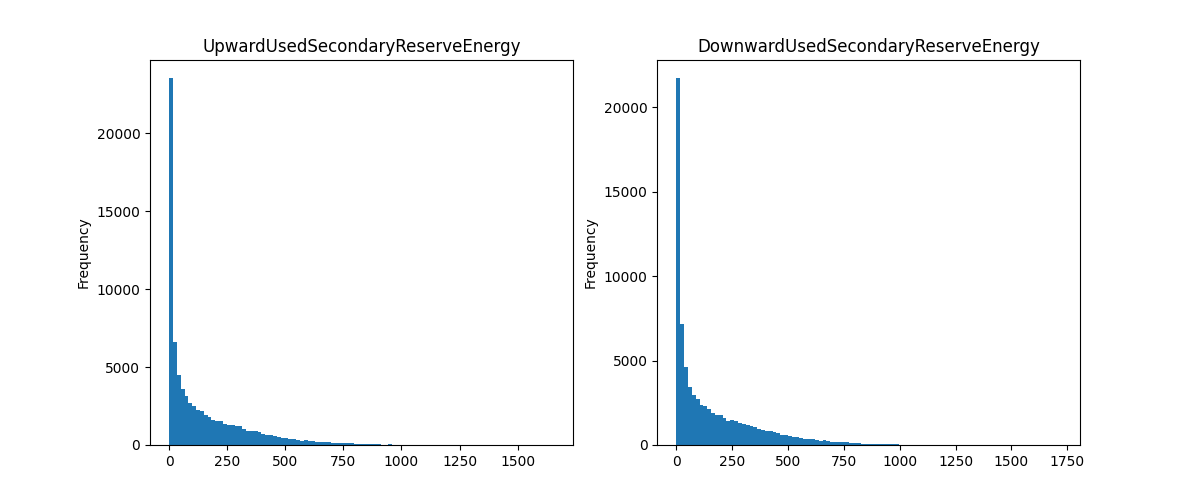
\includegraphics[width=\textwidth]{../plots/target_histograms.png}
  \caption{Frequência dos dados alvos}
\end{figure}


\subsection{Correlações (depth 2)}

Os modelos vão depender bastante de correlação entre variaveis.
Nesta secção queremos tentar identificar se há visiveis relações entre as variaveis, e se há relações temporais  visiveis nas colunas alvo.



\begin{figure}[H]
  \centering
  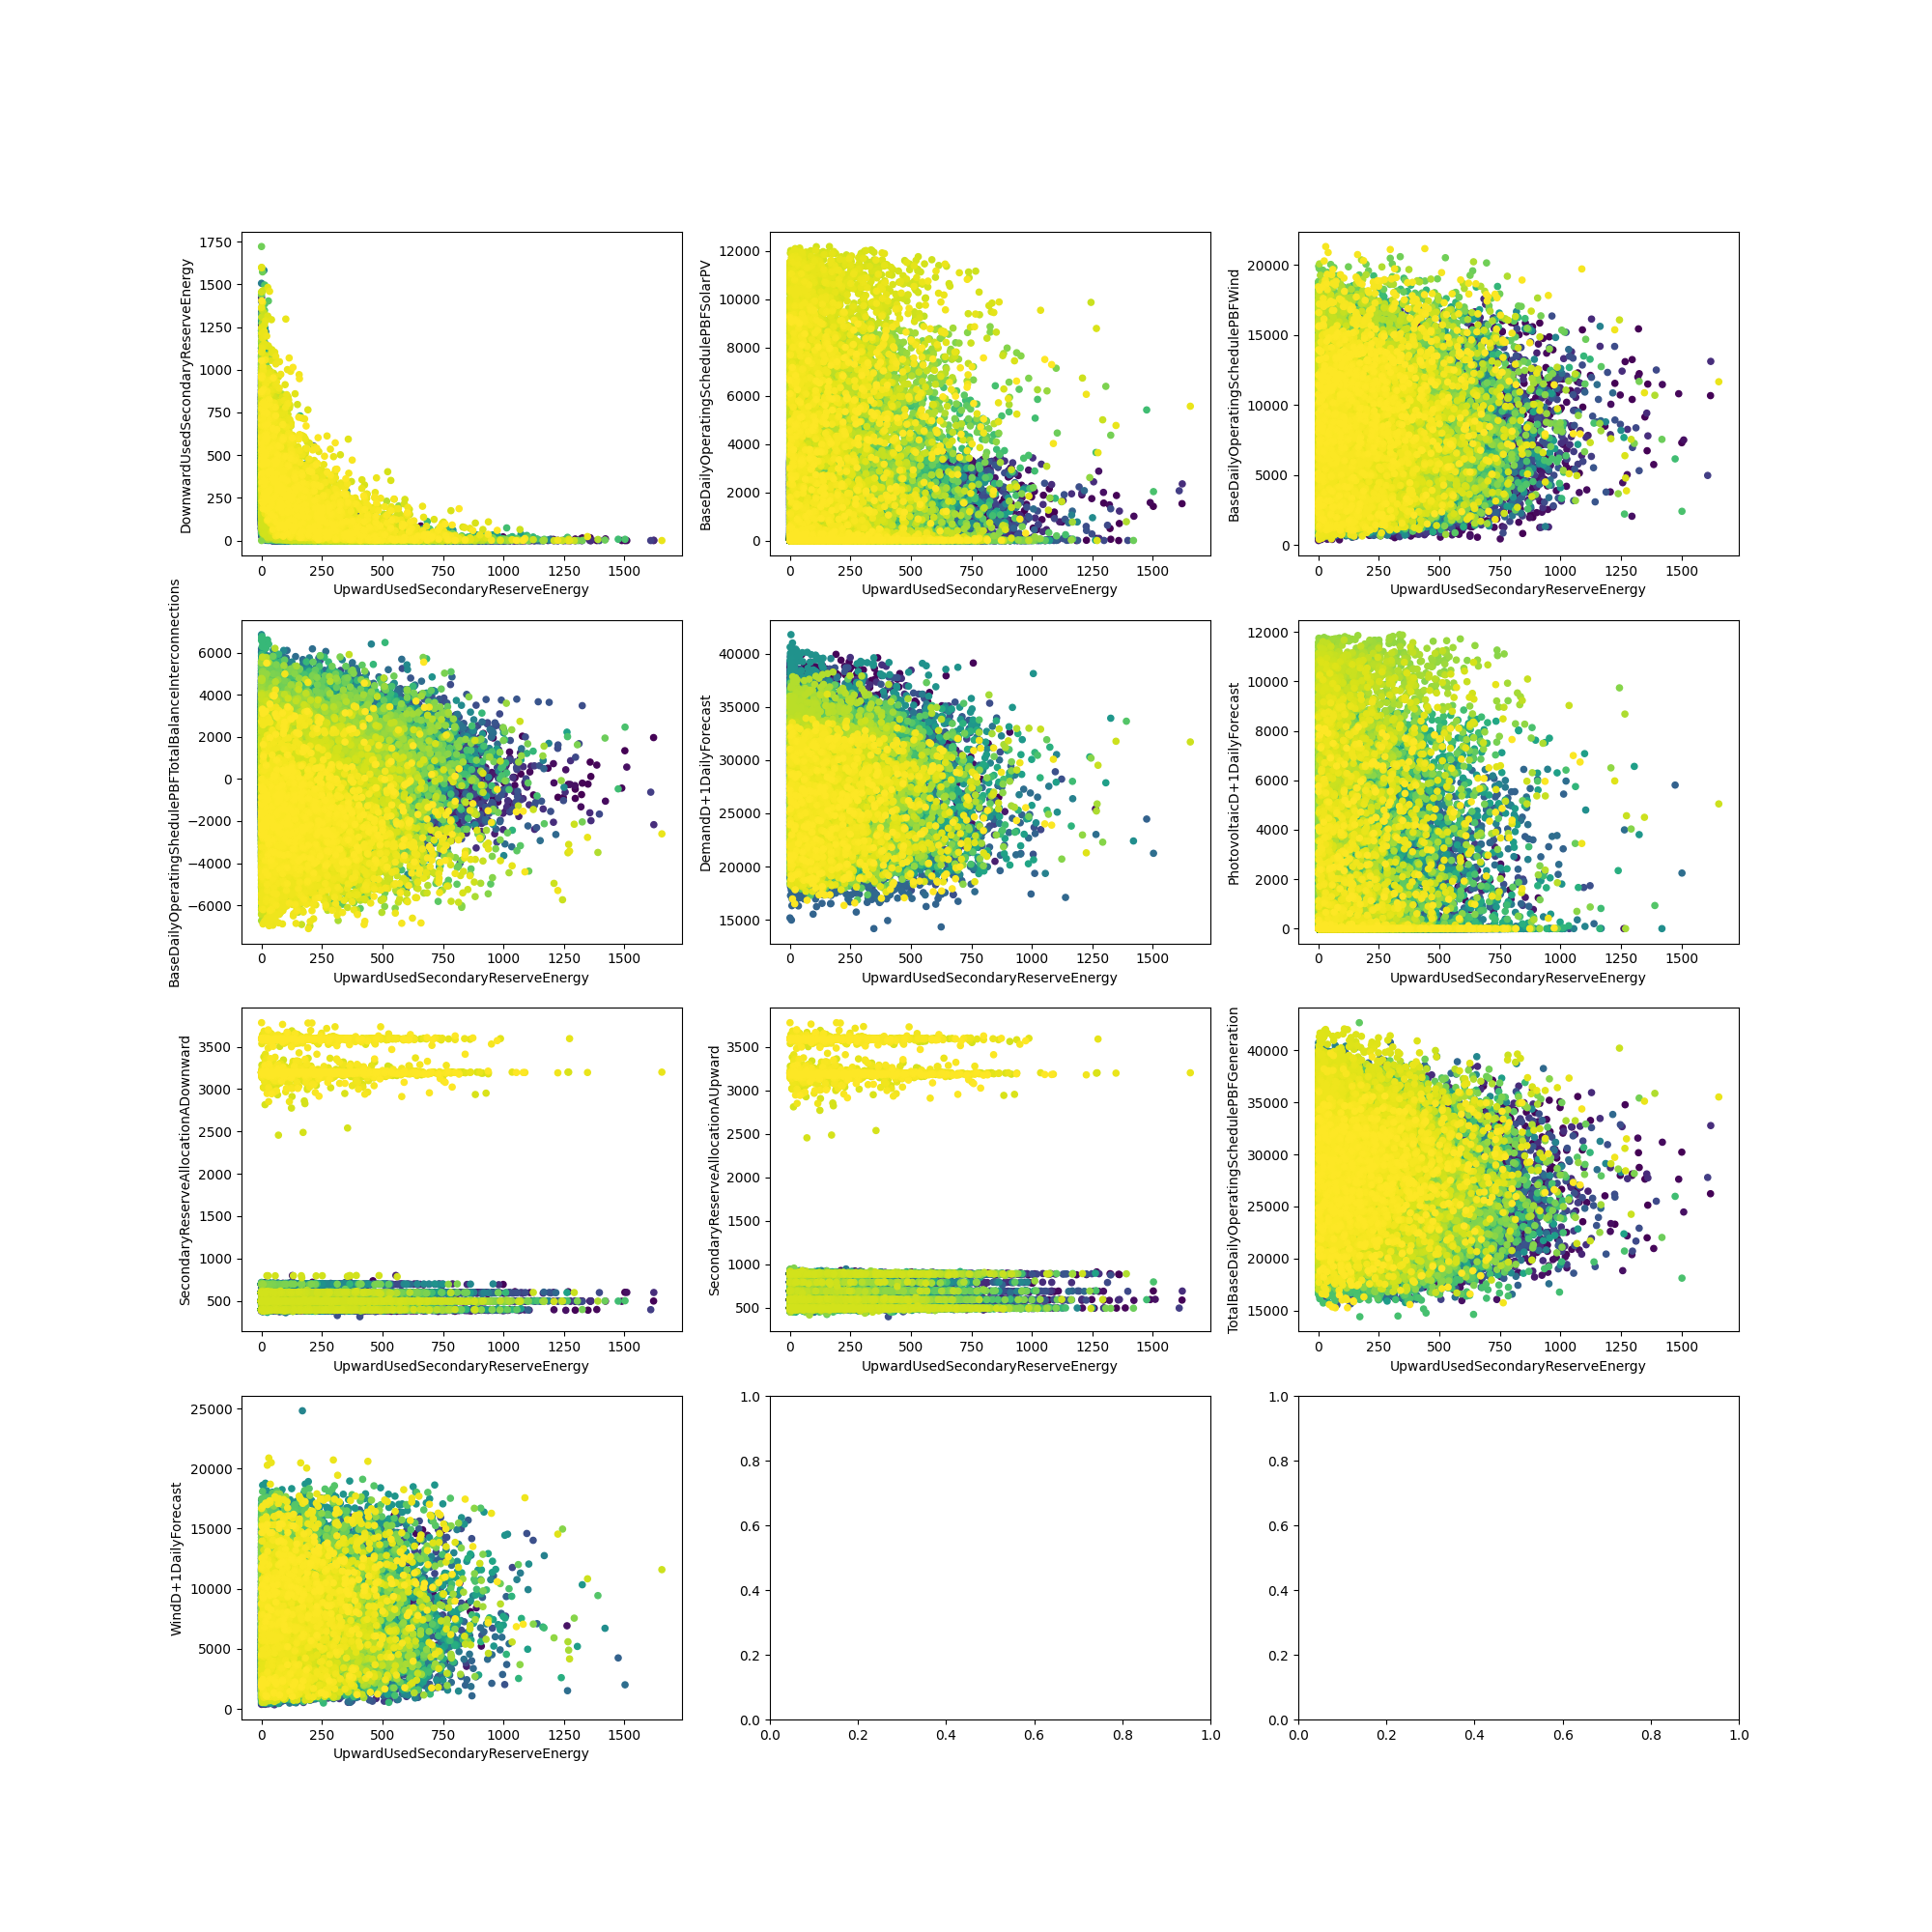
\includegraphics[width=\textwidth]{../plots/feature_correlation.png}
  \caption{Correlação entre atributos}
\end{figure}

As correlações entre variveis parecem muitos escassas o que apresenta já que a previção deste dados usando estas variaveis vai ser um problema dificil.
Por norma é feito uma seleção de  atributos baseado nestas correlações, eliminando assim os atributos que ajudam menos, ou ate prejudicam os modelos.



\begin{figure}[H]
  \centering
  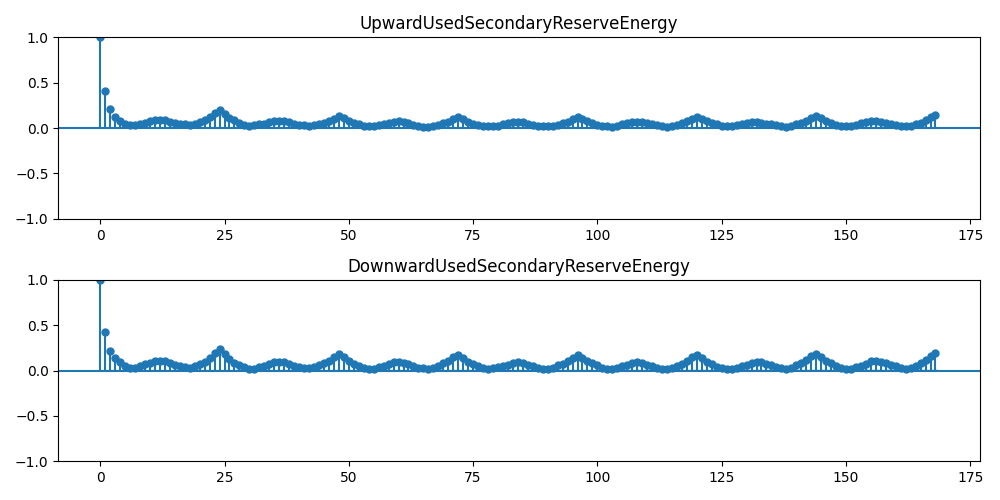
\includegraphics[width=\textwidth]{../plots/autocorrelation.png}
  \caption{Serie Temporal dos dados alvo}
\end{figure}


A autocorrelação, em ambos os "targets", é mais forte nas 3 horas mais proximas, e nos pontos com diferença de 12 e 24 horas.
É de notar que estes valores são baixos, prometendo já tambem uma baixa regressividade temporal.
Outro ponto a denotar é que os objectos não têm um comportamento completamente linear, i.e., parece existir um comportamento discreto na questão ser alocado ou não esta reservas secundárias, e caso seja alocado, aí existir alguma linearidade.
Logo qualquer tipo de modelação terá de resolver primeiramente este problema.

Estas relações mostram que em termos de atributos usados vai ser um desafio complicado para qualquer tipo de modelo.

No âmbito desta disserteção queremos verificar a qualidade das previsões usando estes mesmo atributos, logo, não será feita seleção dos mesmos.

A nível da relação temporal, a maior parte dos modelos que iremos testar aplica um janela na dimensão temporal, usando todos os valores nessa janela, e aplicando os pesos nessas distancias que mais se enquadram. Logo também não é relevante escolher apenas as distancias temporais com maior correlação, pois os modelos vão fazer essa pesagem.

\subsection{Agrupamento \label{se:clustering}}

Uma das possibilidades na modelção será a utilização de grupo de valores, classes, em conjunto com a linearidade.
Devido ao comportamente não exclusivamente linear (tenho de procurar um nome para isto) é tambem estudado as possiveis agregassões (clustering) em que podemos dividir os valores em classe.
Tendo por base que uma das classes é o valor zero, devido ao comportamento não linear desta série, vamos apenas testas quantos, e quais, as melhores classes em que podemos dividir os dados.


preccesos de clsutering elbow e sillpute e merdas, fazer 3 pagindas disto.

clustering
	deu cerca de 15
	5 seria um bom numero de clusters pelos estudos
	mas segundo o tipo de problema 3 + 1(zero) foi o ideal

Ambos os casos apontam um assintota na relação interna dos clusters, a partir de cerca de 5 clusters, sendo que o melhor valor dos verificados seria com 15 clusters.
Para a nossa questão, queremos algumas classes, mas quanto menos classes mais facil será para os modelos correctammente identificar a que classe pertence. Logo para os valores apresentados, escolhemos 5 clusters, sendo que este já pode ser um numero elevado de classes, logo usemos 3 clusters se os modelos tiverem muuita dificuldade com 5.



\section{Tratamento dos dados  \label{se:data_treatment}}

Normalizaçao
A normalizaçao foi deixada por ser aprendida nos modelos, sendo que todos têm como segunda camada, uma de normalização.

Limpeza

Podemos ver pelos graficos seguintes que a existem alguns outliers, sendo estes definidos como 3 desvios padrão de distância à média.

graphhhhhhhhh


No caso de "" e "" existe um grande salto nos valores logo o aqui os dados são partidos e estudados os outliers nas duas diferentes zonas.
A limpeza destes dados é feita apenas substituindo pelo ................................................

Fica também como motivo de estudo se a remoção deste outliers ajuda na modelação.


Estudemos tambem o caso de dados em falta. Alguns destes atributos têm certas entras vazias, e como podemos ver alguns não têm alguns anos inteiros.
Como queremos usar o maximo de dados possiveis iremos usar tecnicas de imputing nesses dados 
............................................
imputing
https://arxiv.org/abs/2102.03340

cleaning
	outliers
		naquela parte que parte fazer a limpeza em duas vezes
		melhora se tirarmos os outliers?
		
	imputing de missing data
	
features adicionais:
	apenas as temporais	

Por ultimo foi adicionado ao dados mais atributos, sendo eles todos de cariz temporal. É adicionado atributos correspondentes à hora, ao dia do ano, ao dia da semana, ao dia do mês, mês, ano. TODO


\section{Considerações adicionais  \label{se:dados_plus}}

Talvez aqui uma secçao para finalizar e mostrar algumas coisas

\label{ch:dados}

% Arquiteturas a estudar
\newpage
\thispagestyle{plain}
\chapter{Arquitecturas de Modelos\label{ch:arquiteturas_modelos}}

Grande parte da literatura sobre previsões em modelos de apredizagem apresenta as mesmas arquiteturas, sendo que são depois aprimoradas consoate os dados e o problema. \\
Apresento aqui as aquiteturas mais usadas em previsões, como tambem algumas usadas noutros ramos tentado prever a compatibilidade neste problema. \\
As arquitecturas irão seguir um esquema logíco comum, um bloco de camadas de entrada, um bloco principal e um por fim um bloco interpretativo. \\
As dimensionalidades destas camadas é o que irá formar as diferentes arquitecturas em estudo. \\

\section{Camadas\label{se:layers}}

Para uma construção de modelos usando a ferramenta \href{https://keras.io/}{keras} a unidade básica são as camadas. Estas representação um operação, com uma entrada, e uma saida, e com possiveis parametrizaçoes específicas. \\
Estas camadas ligadas entre si, perfazem um \"profundo\" de camadas neuronais, chamado profundo pois tem mais  que uma camada. \\

Apresento aqui as camadas utilizadas nos modelos aplicados.

\subsection{Dense\label{se:dense_layer}}

A camada dense pega num input, 

\subsection{Convolution\label{se:conv_layer}}
\subsection{MaxPooling\label{se:max_pooling}}
\subsection{\href{https://keras.io/api/layers/regularization_layers/dropout/}{Dropout}\label{se:dropount}}

Dropout é uma camada que elimina/ignora alguns dos neuronios da camada anterior. Este procedimente impede o overfitting, ajudando na generalização. \\
(ref) na imagem
\begin{figure}[H]
	\centering
	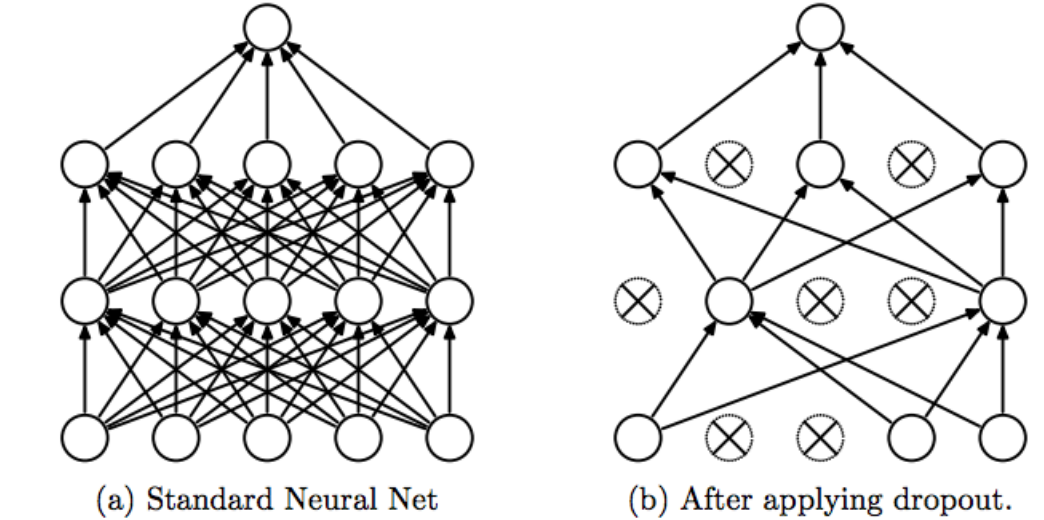
\includegraphics{Imagens/dropout.png}
	\caption{Ilustrção do efeito da camada de dropout}
	\label{fig:dropout}
\end{figure}



\section{Blocos\label{se:blocos}}

Todas as arquiteturas em análise irão ter por base um bloco de camadas neuronais. A formação dessas arquitecturas passa pelas diferentes maneiras que se pode utilizar o bloco principal. Repetições em serie ou em paralelo são um exemplo. \\

\subsection{Bloco Dense\label{se:dense}}

O bloco dense sendo ele o mais simples é formado por duas camadas Dense \cite{}, em que a primeira apresenta um numero maior de filtros que a segunda. \\
Estas camadas não são mais do que uma criação de filtros aleatórios combinando as entradas, para criar todos os filtros de saida. São a base das camadas intrepretativas. A acumulação em série (stacked) de camadas de dense está ligada a melhorias nas capacidades predictivas dos modelos \cite{VLHelen2021}. \\
Exemplo ilustrativo do nosso bloco basico onde entrariam 16 filtros na primeira camada e para finalizar o bloco com 2 filtros \\

\begin{figure}[H]
	\centering
	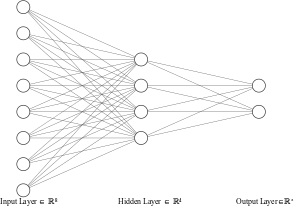
\includegraphics{Imagens/dense_layer.png}
	\caption{Bloco Dense}
	\label{fig:dense_blcok}
\end{figure}
	
\subsection{Blcoo CNN\label{se:cnn}}

Bloco de CNN é aqui definido como uma convolução na dimensão temporal seguido de camadas para combater o overfitting, MaxPooling e Dropout. \\
Normalmente usada em processamentos de imagens, o uso de convuluções temporais é tambem por si mesmo uma ideia forte. \\

explicar om que e CNN
imagem

Usada tambem as ideias de attention, residual e o que eu chamei broad


\subsection{Blcoo LSTM\label{se:lstm}}

O uso de LSTM para previsões é uma area comum, mas aqui é seguido através das ideas partilhas em \cite{Hewamalage2021}, e reforçado pelo uso em previsões energéticas demonstados em \cite{Costa2022} \\
O bloco LSTM é a aplicaçao das RNN, aqui sendo apenas definido como uma camada de LSTM. \\
Estes blocos mantêm dentro de si ligações a diferentes camadas temporais, e cada filtro criado, mantêm uma "memória" dos filtros passados. \\
Bastante utilizado em modelação de linguagem.

imagem


\section{Arquiteturas \label{se:arquitecturas}}

\subsection{Vanilla \label{se:vannila}}

O termo "Vanilla" aqui é aplicado para aquitecturas que apenas usam um bloco de cada, um de entrada, um principal, e um interpretativo. \\
Como exemplo a arquitetura de "VanillaCNN"

imagem da mesma

\subsection{Stacked\label{se:stacked}}

Stacked refere-se a "amontoado" onde se utiliza o bloco principal várias vezes em série.E apenas um bloco de  entrada e um interpretativo. \\
Como exemplo a arquitetura de "StackedCNN"

imagem da mesma

\subsection{MultiHead\label{se:multihea}}

Multihead é o termo para quando os blocos de entrada e principais são repetidos paralelamente, um caminho para cada atributo, ou uma outra paralelização à escolha. Sendo depois concatenadas essas camadas e passadas juntas para a camada interpretativa. \\
Aqui foi usado sempre a paralelização por atributos, e ao invês de fazer Mulithead no sentido de multiplas entradas, para simplicidade de programação, foi feito um paralização interna no modelo, apos a camada de entrada, onde a mesma é repetida para cada atributo. \\
Foi testado a diferença, e para os dados usados não havia diferenças de qualidade, mas sim em tempo de treino, logo a mais rapida foi a escolhida. \\
Como exemplo a arquitetura de "MultiheadCNN"

imagem da mesma

\subsection{MultiTail\label{se:multitail}}

Esta arquitectura tem o mesmo conceito que a anterior a nivel de paralelização, mas neste caso esta é feita apenas na camada interpretativa. Sendo que o resultado do bloco principal é repetido para criar a paralelização. \\
Neste caso foi paralelizado com o numero de tempos a prever, 24 horas, 24 objectos de saida destas modelos.  \\
A grande diferença desta arquitectura para a "Vanilla" que preve 24 horas, é que aqui cada hora tem o seu proprio valor de função de perda, logo o modelo como que está a treinar 24 modelos diferentes, e no caso "Vanilla" a função de perda é ùnica e é a media do erro das horas todas. \\
Como exemplo a arquitetura de "MultiTailCNN"

imagem da mesma

\subsection{UNET\label{se:UNET}}

Normalmente usando em modelção de imagens, a arquitectura UNET passa por criar uma rede de expansão dos filtros, usando convoluções, e de seguida uma rede de contracção dos mesmo, até aos tamanhos pretendidos.\\
O bloco principal contextualmente o mesmo que o CNN.\\
Nas suas ligações UNET junta informação de filtros passados (não de nivel temporal mas de rede neuronal) para realçar informação já trabalhada, e assim identificar padrões de vários contextos diferentes.\\
É habitual tambem adicionar aos blocos principais portões de atenção, portões residuais. Estas duas tecnicas são tambem estudadas aqui.\\
É chamada assim pois é uma rede (NET) que forma um U na sua expansão e contracção.\\

Como exemplo a arquitetura de "UNET"

imagem da mesma


\section{Considerações adicionais\label{se:modelos_plus}}

Aqui e dizer que os modelos utilizados para teste sao as combinacoes deste blocos nestas aquiteturas.

Imagens de layers criadas com 
dense
http://alexlenail.me/NN-SVG/index.html
\label{ch:arch}




% Métodos
\newpage
\thispagestyle{plain}
\chapter{Métodos}

Para responder a primeira questão estudou-se o comportamento do parâmetro p na equação publicada pela ENTSO-E para a Banda de Regulação Secundária a Subir \cite{CMVM2018}:
\begin{equation}
\label{eq:eq_entso-e}
    BRSsubir = p \times \sqrt{a \times Lmax + b^2} - b 
\end{equation}
TODO: explicação das variaveis

Aplicando os dados XXXX (dados históricos do mercado MIBEL), 

Usandos os dados XXXXX para o calculo directo do parâmetro p e comparando com o mesmo parâmetro apresentado na tese de Célia Carneiro \cite{Carneiro2016}, temos a seguinte distribuição de valores:

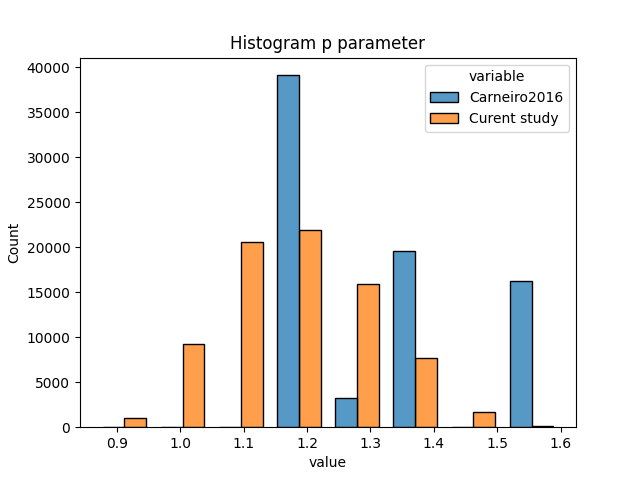
\includegraphics{Imagens/Histogram p parameter.png}
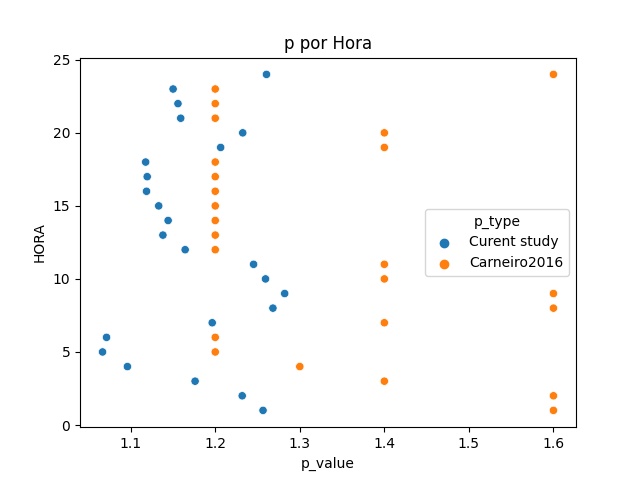
\includegraphics{Imagens/p por Hora.png}

Verifica-se que não têm qualquer relação entre si.

Para a normalização deste parâmetro à Hora, estudou-se o erro entre a Banda a Subir calculada através das normalizações e a Banda a Subir disponível nos dados. 

\begin{table}[H]
\centering
\caption{Isto é um exemplo de uma tabela. Se fôr igual(copiada) a outro autor deve ser pedido autorização para reproduzir.}
\begin{tabular}{p{5cm}p{3.5cm}p{2cm}p{2cm}}
\toprule %thicker line
\textbf{Normalização/Erro} & \textbf{MAE} & \textbf{RMSE} & \textbf{Mediana AE} \\ \hline
\multirow{1}{*}{media}   & 23.03 & 29.15 & 19.04            \\ \hline
\multirow{1}{*}{mediana}   & 22.95 & 29.14 & 18.93            \\ \hline
\multirow{1}{*}{media ponderada}   & 23.39 & 29.57 & 19.28            \\ \hline
\end{tabular}
\end{table}

A normalização que traz erros mais baixos à Banda é a mediana.
Comparando com os p \cite{Carneiro2016}: 

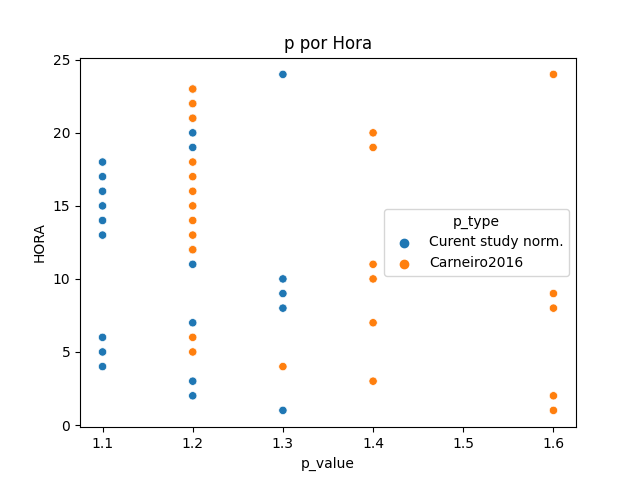
\includegraphics{Imagens/p por Hora norm.png}

Podemos verificar que os valores não coincidem.
Comparando as bandas calculadas:

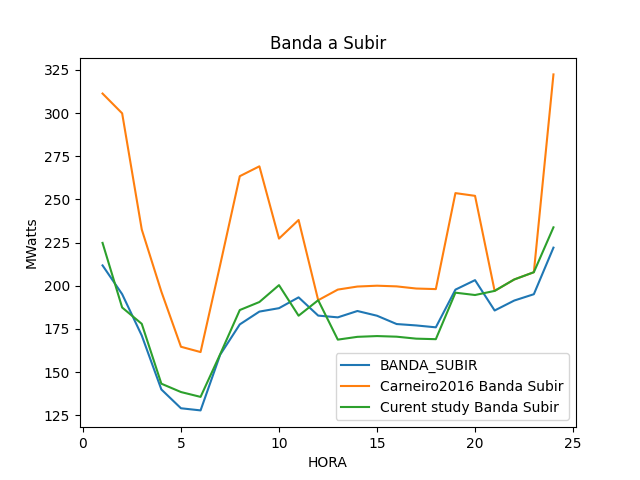
\includegraphics{Imagens/Banda a Subir.png}

Retiramos as médias dos erros percentuais e podemos observar em:

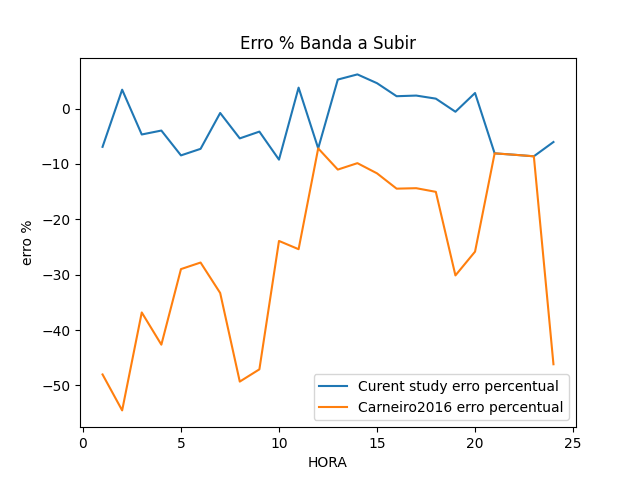
\includegraphics{Imagens/Erro per Banda a Subir.png}

Que conclui que o p calculado agora tem uma prestação bastante mais perto da realidade. 
Onde cerca de 25\% dos casos cai dentro da margem de erro de 5\% na Banda. E na outra tese apenas 10\% cai dentro dessa margem de erro.



Aqui descrever qual o método seguido para responder às perguntas de investigação, o método pode incluir o recurso a uma metodologia reconhecida internacionalmente e já publicada por exemplo numa norma ISO\cite{fet_skaar_2006}.
As figuras e tabelas colocadas devem ser sempre referidas no meio do texto tal como todas as referências que aparecem listadas no fim do documento. 



\section{Modelos estatiscos  \label{se:dados_estudo}}

\subsection{subsection ARIMA (depth 2)}

\subsection{subsubsection Gerador de dados (depth 2)}
distribuiçao

clustering




\section{Forecat  \label{se:dados_estudo}}

\subsection{subsection Construtor de modelos (depth 2)}

\subsection{subsubsection Gerador de dados (depth 2)}
distribuiçao

clustering


\section{Forecat  \label{se:dados_estudo}}

\subsection{subsection Construtor de modelos (depth 2)}

\subsection{subsubsection Gerador de dados (depth 2)}
distribuiçao

clustering



\label{ch:metodos}

% Resultados e discussão
\newpage
\thispagestyle{plain}
\chapter{Resultados e discussão}

Aqui devem constar gráficos e sua análise crítica e ligação com a secção 2 da revisão bibliográfica no sentido de comparar valores e discutir diferenças, por exemplo. A legenda dos gráficos deve seguir a das figuras, isto é, porque também são figuras.

% Para introduzir figuras
\begin{figure}[H]
\centering
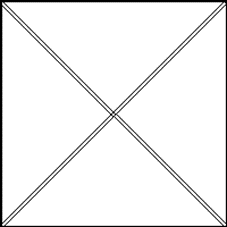
\includegraphics[width=150pt, keepaspectratio]{Imagens/FigA.png}
% legenda da figura por baixo
\caption{Exemplo de como considerar um gráfico}
\label{fig:grafico1} % referência única da figura
\end{figure}

\label{ch:resultados_discussao}

% Conclusões e sugestões futuras
\newpage
\thispagestyle{plain}
\chapter{Conclusões e sugestões futuras}

Aqui são dadas as respostas às perguntas de investigação formuladas na secção \ref{se:objetivos}. Não fazer aqui a discussão dos resultados. Essa discussão deve ser feita no capitulo \ref{ch:resultados_discussao}. Não esquecer de indicar sugestões futuras para que um colega possa dar continuidade ao trabalho desenvolvido. 
\label{ch:conclusao}

% Referências Bibliográficas
\renewcommand{\bibname}{Referências} %comando para rename a BIBLIOGRAFIA para REFERENCIAS
\addcontentsline{toc}{chapter}{\numberline{6}Referências}%
%\bibliographystyle{babplain}      % basic style, author-year citations
\printbibliography

% Referências Bibliográficas
\appendix
\newpage
\thispagestyle{plain}
\chapter{Anexos}

% Para introduzir figuras
\begin{figure}[H]
\centering
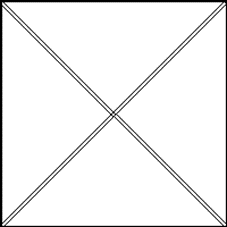
\includegraphics[width=150pt, keepaspectratio]{Imagens/FigA.png}
% legenda da figura por baixo
\caption{Exemplo de como considerar um gráfico nos anexos.}
\label{fig:grafico1} % referência única da figura
\end{figure}

\setlength\tabcolsep{4pt}
\begin{table}[H]
\centering
\caption{Isto é um exemplo de uma tabela. Se fôr igual(copiada) a outro autor deve ser pedido autorização para reproduzir.}
\begin{tabular}{p{5cm}p{3.5cm}p{2cm}p{2cm}}
\toprule %thicker line
\textbf{Title 1} & \textbf{Title 2} & \textbf{Title 3} & \textbf{Title 4} \\ \hline
\multirow{3}{*}{entry 1}   & data      & data    & data             \\
                           & data      & data    & data             \\
                           & data      & data    & data             \\ \hline
\multirow{2}{*}{entry 2}   & data      & data    & data             \\
                           & data      & data    & data             \\ \hline
\multirow{4}{*}{entry 3}   & data      & data    & data             \\
                           & data      & data    & data             \\
                           & data      & data    & data             \\
                           & data      & data    & data             \\ \hline
entry 4                    & data      & data    & data             \\ \hline 
\end{tabular}
\end{table}
\label{ch:Anexos}

\end{document}
